%**************************************%
%*    Generated from PreTeXt source   *%
%*    on 2019-08-01T11:20:20-04:00    *%
%*                                    *%
%*      https://pretextbook.org       *%
%*                                    *%
%**************************************%
\documentclass[oneside,10pt,]{book}
%% Custom Preamble Entries, early (use latex.preamble.early)
%% Default LaTeX packages
%%   1.  always employed (or nearly so) for some purpose, or
%%   2.  a stylewriter may assume their presence
\usepackage{geometry}
%% Some aspects of the preamble are conditional,
%% the LaTeX engine is one such determinant
\usepackage{ifthen}
%% etoolbox has a variety of modern conveniences
\usepackage{etoolbox}
\usepackage{ifxetex,ifluatex}
%% Raster graphics inclusion
\usepackage{graphicx}
%% Color support, xcolor package
%% Always loaded, for: add/delete text, author tools
%% Here, since tcolorbox loads tikz, and tikz loads xcolor
\PassOptionsToPackage{usenames,dvipsnames,svgnames,table}{xcolor}
\usepackage{xcolor}
%% Colored boxes, and much more, though mostly styling
%% skins library provides "enhanced" skin, employing tikzpicture
%% boxes may be configured as "breakable" or "unbreakable"
%% "raster" controls grids of boxes, aka side-by-side
\usepackage{tcolorbox}
\tcbuselibrary{skins}
\tcbuselibrary{breakable}
\tcbuselibrary{raster}
%% We load some "stock" tcolorbox styles that we use a lot
%% Placement here is provisional, there will be some color work also
%% First, black on white, no border, transparent, but no assumption about titles
\tcbset{ bwminimalstyle/.style={size=minimal, boxrule=-0.3pt, frame empty,
colback=white, colbacktitle=white, coltitle=black, opacityfill=0.0} }
%% Second, bold title, run-in to text/paragraph/heading
%% Space afterwards will be controlled by environment,
%% dependent of constructions of the tcb title
\tcbset{ runintitlestyle/.style={fonttitle=\normalfont\bfseries, attach title to upper} }
%% Spacing prior to each exercise, anywhere
\tcbset{ exercisespacingstyle/.style={before skip={1.5ex plus 0.5ex}} }
%% Spacing prior to each block
\tcbset{ blockspacingstyle/.style={before skip={2.0ex plus 0.5ex}} }
%% xparse allows the construction of more robust commands,
%% this is a necessity for isolating styling and behavior
%% The tcolorbox library of the same name loads the base library
\tcbuselibrary{xparse}
%% Hyperref should be here, but likes to be loaded late
%%
%% Inline math delimiters, \(, \), need to be robust
%% 2016-01-31:  latexrelease.sty  supersedes  fixltx2e.sty
%% If  latexrelease.sty  exists, bugfix is in kernel
%% If not, bugfix is in  fixltx2e.sty
%% See:  https://tug.org/TUGboat/tb36-3/tb114ltnews22.pdf
%% and read "Fewer fragile commands" in distribution's  latexchanges.pdf
\IfFileExists{latexrelease.sty}{}{\usepackage{fixltx2e}}
%% Footnote counters and part/chapter counters are manipulated
%% April 2018:  chngcntr  commands now integrated into the kernel,
%% but circa 2018/2019 the package would still try to redefine them,
%% so we need to do the work of loading conditionally for old kernels.
%% From version 1.1a,  chngcntr  should detect defintions made by LaTeX kernel.
\ifdefined\counterwithin
\else
    \usepackage{chngcntr}
\fi
%% Text height identically 9 inches, text width varies on point size
%% See Bringhurst 2.1.1 on measure for recommendations
%% 75 characters per line (count spaces, punctuation) is target
%% which is the upper limit of Bringhurst's recommendations
\geometry{letterpaper,total={340pt,9.0in}}
%% Custom Page Layout Adjustments (use latex.geometry)
%% This LaTeX file may be compiled with pdflatex, xelatex, or lualatex executables
%% LuaTeX is not explicitly supported, but we do accept additions from knowledgeable users
%% The conditional below provides  pdflatex  specific configuration last
%% The following provides engine-specific capabilities
%% Generally, xelatex is necessary non-Western fonts
\ifthenelse{\boolean{xetex} \or \boolean{luatex}}{%
%% begin: xelatex and lualatex-specific configuration
\ifxetex\usepackage{xltxtra}\fi
%% realscripts is the only part of xltxtra relevant to lualatex 
\ifluatex\usepackage{realscripts}\fi
%% fontspec package provides extensive control of system fonts,
%% meaning *.otf (OpenType), and apparently *.ttf (TrueType)
%% that live *outside* your TeX/MF tree, and are controlled by your *system*
%% fontspec will make Latin Modern (lmodern) the default font
\usepackage{fontspec}
%% 
%% Extensive support for other languages
\usepackage{polyglossia}
%% Set main/default language based on pretext/@xml:lang value
%% document language code is "en-US", US English
%% usmax variant has extra hypenation
\setmainlanguage[variant=usmax]{english}
%% Enable secondary languages based on discovery of @xml:lang values
%% Enable fonts/scripts based on discovery of @xml:lang values
%% Western languages should be ably covered by Latin Modern Roman
%% end: xelatex and lualatex-specific configuration
}{%
%% begin: pdflatex-specific configuration
\usepackage[utf8]{inputenc}
%% PreTeXt will create a UTF-8 encoded file
%% begin: font setup and configuration for use with pdflatex
\usepackage{lmodern}
\usepackage[T1]{fontenc}
%% end: font setup and configuration for use with pdflatex
%% end: pdflatex-specific configuration
}
%% Symbols, align environment, bracket-matrix
\usepackage{amsmath}
\usepackage{amssymb}
%% allow page breaks within display mathematics anywhere
%% level 4 is maximally permissive
%% this is exactly the opposite of AMSmath package philosophy
%% there are per-display, and per-equation options to control this
%% split, aligned, gathered, and alignedat are not affected
\allowdisplaybreaks[4]
%% allow more columns to a matrix
%% can make this even bigger by overriding with  latex.preamble.late  processing option
\setcounter{MaxMatrixCols}{30}
%%
%%
%% Division Titles, and Page Headers/Footers
%% titlesec package, loading "titleps" package cooperatively
%% See code comments about the necessity and purpose of "explicit" option
\usepackage[explicit, pagestyles]{titlesec}
\newtitlemark{\chaptertitlename}
%% Set global/default page style for document due
%% to potential re-definitions after documentclass
\pagestyle{headings}
%%
%% Create globally-available macros to be provided for style writers
%% These are redefined for each occurence of each division
\newcommand{\divisionnameptx}{\relax}%
\newcommand{\titleptx}{\relax}%
\newcommand{\subtitleptx}{\relax}%
\newcommand{\shortitleptx}{\relax}%
\newcommand{\authorsptx}{\relax}%
\newcommand{\epigraphptx}{\relax}%
%% Create environments for possible occurences of each division
%% Environment for a PTX "preface" at the level of a LaTeX "chapter"
\NewDocumentEnvironment{preface}{mmmmmm}
{%
\renewcommand{\divisionnameptx}{Preface}%
\renewcommand{\titleptx}{#1}%
\renewcommand{\subtitleptx}{#2}%
\renewcommand{\shortitleptx}{#3}%
\renewcommand{\authorsptx}{#4}%
\renewcommand{\epigraphptx}{#5}%
\chapter*{#1}%
\addcontentsline{toc}{chapter}{#3}
\label{#6}%
}{}%
%% Environment for a PTX "chapter" at the level of a LaTeX "chapter"
\NewDocumentEnvironment{chapterptx}{mmmmmm}
{%
\renewcommand{\divisionnameptx}{Chapter}%
\renewcommand{\titleptx}{#1}%
\renewcommand{\subtitleptx}{#2}%
\renewcommand{\shortitleptx}{#3}%
\renewcommand{\authorsptx}{#4}%
\renewcommand{\epigraphptx}{#5}%
\chapter[#3]{#1}%
\label{#6}%
}{}%
%% Environment for a PTX "section" at the level of a LaTeX "section"
\NewDocumentEnvironment{sectionptx}{mmmmmm}
{%
\renewcommand{\divisionnameptx}{Section}%
\renewcommand{\titleptx}{#1}%
\renewcommand{\subtitleptx}{#2}%
\renewcommand{\shortitleptx}{#3}%
\renewcommand{\authorsptx}{#4}%
\renewcommand{\epigraphptx}{#5}%
\section[#3]{#1}%
\label{#6}%
}{}%
%% Environment for a PTX "subsection" at the level of a LaTeX "subsection"
\NewDocumentEnvironment{subsectionptx}{mmmmmm}
{%
\renewcommand{\divisionnameptx}{Subsection}%
\renewcommand{\titleptx}{#1}%
\renewcommand{\subtitleptx}{#2}%
\renewcommand{\shortitleptx}{#3}%
\renewcommand{\authorsptx}{#4}%
\renewcommand{\epigraphptx}{#5}%
\subsection[#3]{#1}%
\label{#6}%
}{}%
%% Environment for a PTX "exercises" at the level of a LaTeX "subsection"
\NewDocumentEnvironment{exercises-subsection}{mmmmmm}
{%
\renewcommand{\divisionnameptx}{Exercises}%
\renewcommand{\titleptx}{#1}%
\renewcommand{\subtitleptx}{#2}%
\renewcommand{\shortitleptx}{#3}%
\renewcommand{\authorsptx}{#4}%
\renewcommand{\epigraphptx}{#5}%
\subsection[#3]{#1}%
\label{#6}%
}{}%
%% Environment for a PTX "exercises" at the level of a LaTeX "subsection"
\NewDocumentEnvironment{exercises-subsection-numberless}{mmmmmm}
{%
\renewcommand{\divisionnameptx}{Exercises}%
\renewcommand{\titleptx}{#1}%
\renewcommand{\subtitleptx}{#2}%
\renewcommand{\shortitleptx}{#3}%
\renewcommand{\authorsptx}{#4}%
\renewcommand{\epigraphptx}{#5}%
\subsection*{#1}%
\addcontentsline{toc}{subsection}{#3}
\label{#6}%
}{}%
%% Environment for a PTX "index" at the level of a LaTeX "chapter"
\NewDocumentEnvironment{indexptx}{mmmmmm}
{%
\renewcommand{\divisionnameptx}{Index}%
\renewcommand{\titleptx}{#1}%
\renewcommand{\subtitleptx}{#2}%
\renewcommand{\shortitleptx}{#3}%
\renewcommand{\authorsptx}{#4}%
\renewcommand{\epigraphptx}{#5}%
\chapter*{#1}%
\addcontentsline{toc}{chapter}{#3}
\label{#6}%
}{}%
%%
%% Styles for six traditional LaTeX divisions
\titleformat{\chapter}[display]
{\normalfont\huge\bfseries}{\divisionnameptx\space\thechapter}{20pt}{\Huge#1}
[{\Large\authorsptx}]
\titleformat{name=\chapter,numberless}[display]
{\normalfont\huge\bfseries}{}{0pt}{#1}
[{\Large\authorsptx}]
\titlespacing*{\chapter}{0pt}{50pt}{40pt}
\titleformat{\section}[hang]
{\normalfont\Large\bfseries}{\thesection}{1ex}{#1}
[{\large\authorsptx}]
\titleformat{name=\section,numberless}[block]
{\normalfont\Large\bfseries}{}{0pt}{#1}
[{\large\authorsptx}]
\titlespacing*{\section}{0pt}{3.5ex plus 1ex minus .2ex}{2.3ex plus .2ex}
\titleformat{\subsection}[hang]
{\normalfont\large\bfseries}{\thesubsection}{1ex}{#1}
[{\normalsize\authorsptx}]
\titleformat{name=\subsection,numberless}[block]
{\normalfont\large\bfseries}{}{0pt}{#1}
[{\normalsize\authorsptx}]
\titlespacing*{\subsection}{0pt}{3.25ex plus 1ex minus .2ex}{1.5ex plus .2ex}
\titleformat{\subsubsection}[hang]
{\normalfont\normalsize\bfseries}{\thesubsubsection}{1em}{#1}
[{\small\authorsptx}]
\titleformat{name=\subsubsection,numberless}[block]
{\normalfont\normalsize\bfseries}{}{0pt}{#1}
[{\normalsize\authorsptx}]
\titlespacing*{\subsubsection}{0pt}{3.25ex plus 1ex minus .2ex}{1.5ex plus .2ex}
\titleformat{\paragraph}[hang]
{\normalfont\normalsize\bfseries}{\theparagraph}{1em}{#1}
[{\small\authorsptx}]
\titleformat{name=\paragraph,numberless}[block]
{\normalfont\normalsize\bfseries}{}{0pt}{#1}
[{\normalsize\authorsptx}]
\titlespacing*{\paragraph}{0pt}{3.25ex plus 1ex minus .2ex}{1.5em}
%%
%% Semantic Macros
%% To preserve meaning in a LaTeX file
%%
%% \mono macro for content of "c", "cd", "tag", etc elements
%% Also used automatically in other constructions
%% Simply an alias for \texttt
%% Always defined, even if there is no need, or if a specific tt font is not loaded
\newcommand{\mono}[1]{\texttt{#1}}
%%
%% Following semantic macros are only defined here if their
%% use is required only in this specific document
%%
%% Used for inline definitions of terms
\newcommand{\terminology}[1]{\textbf{#1}}
%% Division Numbering: Chapters, Sections, Subsections, etc
%% Division numbers may be turned off at some level ("depth")
%% A section *always* has depth 1, contrary to us counting from the document root
%% The latex default is 3.  If a larger number is present here, then
%% removing this command may make some cross-references ambiguous
%% The precursor variable $numbering-maxlevel is checked for consistency in the common XSL file
\setcounter{secnumdepth}{3}
%% begin: General AMS environment setup
%% Environments built with amsthm package
\usepackage{amsthm}
%% Numbering for Theorems, Conjectures, Examples, Figures, etc
%% Controlled by  numbering.theorems.level  processing parameter
%% Numbering: all theorem-like numbered consecutively
%% i.e. Corollary 4.3 follows Theorem 4.2
%% Always need some theorem environment to set base numbering scheme
%% even if document has no theorems (but has other environments)
%% Create a never-used style first, always
%% simply to provide a global counter to use, namely "cthm"
\newtheorem{cthm}{BadTheoremStringName}[section]
%% AMS "proof" environment is not used, but we leave previously
%% implemented \qedhere in place, should the LaTeX be recycled
\renewcommand{\qedhere}{\relax}
%% end: General AMS environment setup
%%
%% xparse environments for introductions and conclusions of divisions
%%
%% introduction: in a structured division
\NewDocumentEnvironment{introduction}{m}
{\notblank{#1}{\noindent\textbf{#1}\space}{}}{\par\medskip}
%%
%% tcolorbox, with styles, for miscellaneous environments
%%
%% assemblage: fairly simple un-numbered block/structure
\tcbset{ assemblagestyle/.style={size=normal, colback=white, colbacktitle=white, coltitle=black, colframe=black, rounded corners, titlerule=0.0pt, center title, fonttitle=\normalfont\bfseries, blockspacingstyle, } }
\newtcolorbox{assemblage}[2]{title={\notblank{#1}{#1}{}}, phantomlabel={#2}, breakable, parbox=false, assemblagestyle}
%% Divisional exercises (and worksheet) as LaTeX environments
%% Third argument is option for extra workspace in worksheets
%% Hanging indent occupies a 5ex width slot prior to left margin
%% Experimentally this seems just barely sufficient for a bold "888."
%% Division exercises, not in exercise group
\tcbset{ divisionexercisestyle/.style={bwminimalstyle, runintitlestyle, exercisespacingstyle, left=5ex, breakable, parbox=false } }
\newtcolorbox{divisionexercise}[4]{divisionexercisestyle, before title={\hspace{-5ex}\makebox[5ex][l]{#1.}}, title={\notblank{#2}{#2\space}{}}, phantom={\hypertarget{#4}{}}, after={\notblank{#3}{\newline\rule{\workspacestrutwidth}{#3\textheight}\newline}{}}}
%% Localize LaTeX supplied names (possibly none)
\renewcommand*{\chaptername}{Chapter}
\setcounter{chapter}{-1}
%% Equation Numbering
%% Controlled by  numbering.equations.level  processing parameter
%% No adjustment here implies document-wide numbering
\numberwithin{equation}{section}
%% "tcolorbox" environment for a single image, occupying entire \linewidth
%% arguments are left-margin, width, right-margin, as multiples of
%% \linewidth, and are guaranteed to be positive and sum to 1.0
\tcbset{ imagestyle/.style={bwminimalstyle} }
\NewTColorBox{image}{mmm}{imagestyle,left skip=#1\linewidth,width=#2\linewidth}
%% Figures, Tables, Listings, Named Lists, Floats
%% The [H]ere option of the float package fixes floats in-place,
%% in deference to web usage, where floats are totally irrelevant
%% You can remove some of this setup, to restore standard LaTeX behavior
%% HOWEVER, numbering of figures/tables AND theorems/examples/remarks, etc
%% may de-synchronize with the numbering in the HTML version
%% You can remove the "placement={H}" option to allow flotation and
%% preserve numbering, BUT the numbering may then appear "out-of-order"
%% Floating environments: http://tex.stackexchange.com/questions/95631/
\usepackage{float}
\usepackage{newfloat}
\usepackage{caption}%% Adjust stock figure environment so that it no longer floats
\SetupFloatingEnvironment{figure}{fileext=lof,placement={H},within=section,name=Figure}
\captionsetup[figure]{labelfont=bf,justification=raggedright}
%% http://tex.stackexchange.com/questions/16195
\makeatletter
\let\c@figure\c@cthm
\makeatother
%% Footnote Numbering
%% Specified by numbering.footnotes.level
%% Undo counter reset by chapter for a book
\counterwithout{footnote}{chapter}
\counterwithin*{footnote}{section}
%% More flexible list management, esp. for references
%% But also for specifying labels (i.e. custom order) on nested lists
\usepackage{enumitem}
%% Support for index creation
%% imakeidx package does not require extra pass (as with makeidx)
%% Title of the "Index" section set via a keyword
%% Language support for the "see" and "see also" phrases
\usepackage{imakeidx}
\makeindex[title=Index, intoc=true]
\renewcommand{\seename}{See}
\renewcommand{\alsoname}{See also}
%% hyperref driver does not need to be specified, it will be detected
%% Footnote marks in tcolorbox have broken linking under
%% hyperref, so it is necessary to turn off all linking
%% It *must* be given as a package option, not with \hypersetup
\usepackage[hyperfootnotes=false]{hyperref}
%% Hyperlinking active in electronic PDFs, all links solid and blue
\hypersetup{colorlinks=true,linkcolor=blue,citecolor=blue,filecolor=blue,urlcolor=blue}
\hypersetup{pdftitle={Introduction to Modern Algebra and Geometry}}
%% If you manually remove hyperref, leave in this next command
\providecommand\phantomsection{}
%% Graphics Preamble Entries
\usepackage{pgfplots}               % loads tikz package
        \usepackage{smartdiagram}           % for a circular diagram
\pgfplotsset{axis x line = middle,
axis y line = middle}
\usetikzlibrary{backgrounds}
\usetikzlibrary{arrows,matrix}
        \usetikzlibrary{positioning}        % for Dave R's worksheet
        \usepackage{circuitikz}             % for Virgil P's worksheet
%% If tikz has been loaded, replace ampersand with \amp macro
%% extpfeil package for certain extensible arrows,
%% as also provided by MathJax extension of the same name
%% NB: this package loads mtools, which loads calc, which redefines
%%     \setlength, so it can be removed if it seems to be in the 
%%     way and your math does not use:
%%     
%%     \xtwoheadrightarrow, \xtwoheadleftarrow, \xmapsto, \xlongequal, \xtofrom
%%     
%%     we have had to be extra careful with variable thickness
%%     lines in tables, and so also load this package late
\usepackage{extpfeil}
%% Custom Preamble Entries, late (use latex.preamble.late)
%% Begin: Author-provided packages
%% (From  docinfo/latex-preamble/package  elements)
\usepackage{tikz}\usepackage{graphicx}%% End: Author-provided packages
%% Begin: Author-provided macros
%% (From  docinfo/macros  element)
%% Plus three from MBX for XML characters
\DeclareMathOperator{\re}{Re}
\DeclareMathOperator{\im}{Im}
\DeclareMathOperator{\Aut}{Aut}
\newcommand{\C}{{\rm \bf C}}
\newcommand{\R}{{\rm \bf R}}
\newcommand{\lt}{<}
\newcommand{\gt}{>}
\newcommand{\amp}{&}
%% End: Author-provided macros
\begin{document}
\frontmatter
%% begin: half-title
\thispagestyle{empty}
{\centering
\vspace*{0.28\textheight}
{\Huge Introduction to Modern Algebra and Geometry}\\}
\clearpage
%% end:   half-title
%% begin: adcard
\thispagestyle{empty}
\null%
\clearpage
%% end:   adcard
%% begin: title page
%% Inspired by Peter Wilson's "titleDB" in "titlepages" CTAN package
\thispagestyle{empty}
{\centering
\vspace*{0.14\textheight}
%% Target for xref to top-level element is ToC
\addtocontents{toc}{\protect\hypertarget{x:book:algeom_text}{}}
{\Huge Introduction to Modern Algebra and Geometry}\\[3\baselineskip]
{\Large David W. Lyons}\\[0.5\baselineskip]
{\Large Lebanon Valley College\\
Annville, PA, USA}\\[3\baselineskip]
{\Large August 1, 2019}\\}
\clearpage
%% end:   title page
%% begin: copyright-page
\thispagestyle{empty}
\vspace*{\stretch{2}}
\vspace*{\stretch{1}}
\null\clearpage
%% end:   copyright-page
Abstract blurb goes here.%
%
%
\typeout{************************************************}
\typeout{Preface  Preface}
\typeout{************************************************}
%
\begin{preface}{Preface}{}{Preface}{}{}{g:preface:idp140657217959344}
This is a short sentence. And some more. A few words about the purpose, aim, and scope of these notes.%
%
\begin{equation*}
x^2 + e^3 = 7
\end{equation*}
\end{preface}
%% begin: table of contents
%% Adjust Table of Contents
\setcounter{tocdepth}{1}
\renewcommand*\contentsname{Contents}
\tableofcontents
%% end:   table of contents
\mainmatter
%
%
\typeout{************************************************}
\typeout{Chapter 0 Basics}
\typeout{************************************************}
%
\begin{chapterptx}{Basics}{}{Basics}{}{}{x:chapter:basics_chapter}
\begin{introduction}{}%
This chapter is about some basics.\end{introduction}%
%
%
\typeout{************************************************}
\typeout{Section 0.1 Complex Numbers}
\typeout{************************************************}
%
\begin{sectionptx}{Complex Numbers}{}{Complex Numbers}{}{}{g:section:idp140657235264848}
\begin{introduction}{}%
The set of complex numbers, denoted \(\C\), is in one-to-one correspondence with the 2-dimensional real plane \(\R^2\). We will write \(z\leftrightarrow (x,y)\) to denote that the complex number \(z\) corresponds to the ordered pair \((x,y)\) of real numbers.%
\end{introduction}%
%
%
\typeout{************************************************}
\typeout{Subsection 0.1.1 Real and imaginary parts}
\typeout{************************************************}
%
\begin{subsectionptx}{Real and imaginary parts}{}{Real and imaginary parts}{}{}{g:subsection:idp140657235272144}
Given a complex number \(z\) corresponding to the point \((x,y)\) in \(\R^2\), we say that \(x\) is the \terminology{real part} of \(z\) and that \(y\) is the \terminology{imaginary part} of \(z\), denoted \(\re(z)=x\) and \(\im(z)=y\). The complex numbers contain the real numbers \(\R\) as a subset. The real number \(x\), which is also the complex number \(x\), corresponds to the ordered pair \((x,0)\), The complex number \(i\) corresponds to the ordered pair \((0,1)\). Here is a summary so far.%
%
\begin{align*}
z \amp \leftrightarrow (\re(z),\im(z))\\
x\in \R \amp \leftrightarrow (x,0)\\
i \amp \leftrightarrow (0,1)
\end{align*}
\end{subsectionptx}
%
%
\typeout{************************************************}
\typeout{Subsection 0.1.2 Modulus and argument}
\typeout{************************************************}
%
\begin{subsectionptx}{Modulus and argument}{}{Modulus and argument}{}{}{g:subsection:idp140657216848192}
Given a complex number \(z\leftrightarrow (x,y)\), let \((r,\theta)\) be polar coordinates for the point \((x,y)\) such that \(r\geq 0\) and \(\theta\) is measured in radians. The \terminology{modulus} or \terminology{norm} of \(z\), denoted \(|z|\), is defined to be the polar coordinate \(r=\sqrt{x^2+y^2}\) and the \terminology{argument} of \(z\), denoted \(\arg{z}\), is the polar coordinate \(\theta\), that is, the oriented angle made by the real vector \((x,y)\) with the positive real axis. In other words, \((|z|,\arg{z})\) are polar coordinates for the point \((x,y)\). Here is a summary.%
\begin{assemblage}{Norm and argument.}{g:assemblage:idp140657216858336}%
%
\begin{equation}
z\leftrightarrow (x,y) = \left(|z|\cos( \arg{z}),|z|\sin(\arg{z})\right) \label{x:men:normargdef}
\end{equation}
%
\end{assemblage}
\end{subsectionptx}
%
%
\typeout{************************************************}
\typeout{Subsection 0.1.3 Addition and multiplication of complex numbers}
\typeout{************************************************}
%
\begin{subsectionptx}{Addition and multiplication of complex numbers}{}{Addition and multiplication of complex numbers}{}{}{g:subsection:idp140657216883584}
Given complex numbers \(z\leftrightarrow (x,y)\) and \(z'\leftrightarrow
(x',y')\), the sum \(z+z'\) is defined by the following.%
\begin{assemblage}{Complex addition.}{g:assemblage:idp140657216792208}%
%
\begin{equation}
z+z' \leftrightarrow (x+x',y+y')\label{x:men:complexadddef}
\end{equation}
%
\end{assemblage}
In other words, complex addition corresponds to real vector addition. See Figure \hyperref[x:figure:parallelogramlawfig]{Figure~\ref{x:figure:parallelogramlawfig}}. \begin{figure}
\centering
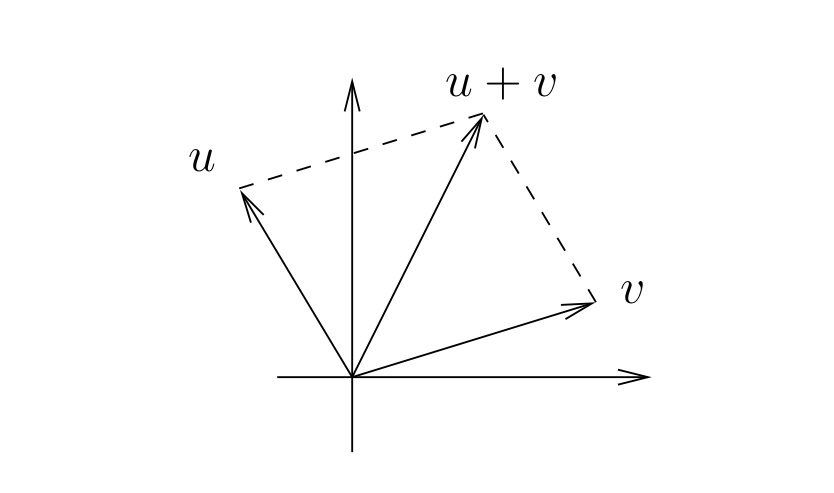
\includegraphics[width=0.6\linewidth]{images/parallelogramlaw_clip.jpg}
\caption{Complex addition is vector addition\label{x:figure:parallelogramlawfig}}
\end{figure}
%
\par
The product \(zz'\) is defined as follows.%
\begin{assemblage}{Complex multiplication.}{g:assemblage:idp140657216823920}%
%
\begin{align}
|zz'| \amp = |z||z'|\label{x:mrow:complexmultdefnorm}\\
\arg(zz') \amp = \arg{z}+\arg{z'}\label{x:mrow:complexmultdefarg}
\end{align}
%
\end{assemblage}
The interaction between complex addition and multiplication is expressed by the following relationship, which holds for any complex \(z,u,v\). See Figure \hyperref[x:figure:distlawfig]{Figure~\ref{x:figure:distlawfig}}.%
\begin{assemblage}{Distributive law.}{g:assemblage:idp140657216799312}%
%
\begin{equation}
z(u+v) = zu+zv \label{x:men:distributivelaw}
\end{equation}
%
\end{assemblage}
\begin{figure}
\centering
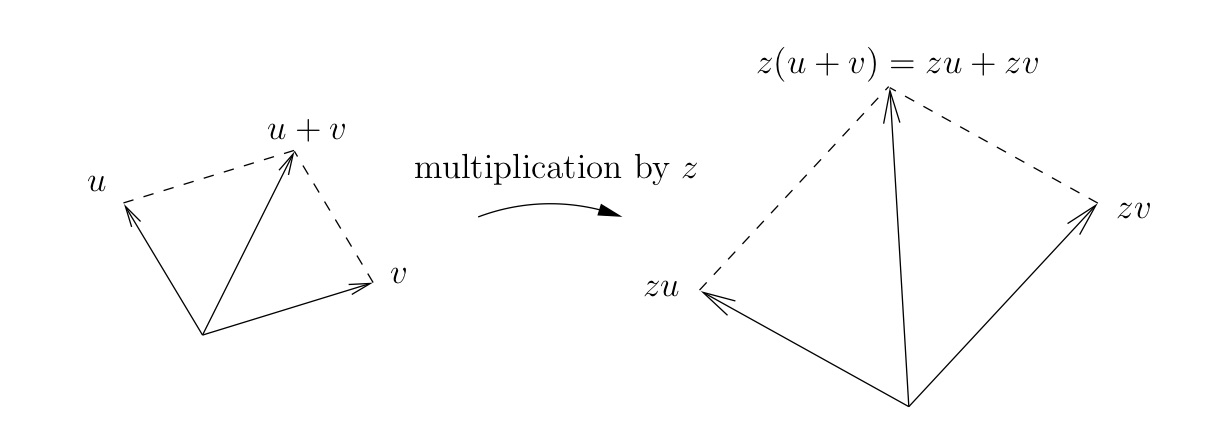
\includegraphics[width=1\linewidth]{images/distlaw_clip.jpg}
\caption{The distributive law: multiplication by \(z\) rotates the vectors \(u\), \(v\), and \(u+v\) by angle \(\arg z\) and scales by the factor \(|z|\). The sum of the rotated vectors \(u,v\) is the rotated sum vector.\label{x:figure:distlawfig}}
\end{figure}
Below are a number of relationships arising from the definitions of complex addition and multiplication. Let \(a,b,c,d\) be real numbers and let \(z,u,v\) be complex numbers. The following relationships hold. \footnote{Equations \hyperref[x:mrow:addextends]{(\ref{x:mrow:addextends})}, \hyperref[x:mrow:multextends]{(\ref{x:mrow:multextends})}, and \hyperref[x:mrow:normextends]{(\ref{x:mrow:normextends})} say that complex addition, multiplication, and norm \emph{extend} the corresponding operations on the reals. Equation \hyperref[x:mrow:multidentity]{(\ref{x:mrow:multidentity})} is expressed by saying 1 is the \emph{multiplicative identity}.\label{g:fn:idp140657216817728}}%
\begin{align}
a+ib \amp \leftrightarrow (a,b)\label{g:mrow:idp140657216854976}\\
a+b \;\;\text{(complex sum)} \amp= a+b \;\;\text{(real sum)}\label{x:mrow:addextends}\\
ab \;\;\text{(complex product)} \amp = ab \;\;\text{(real product)}\label{x:mrow:multextends}\\
|a| \;\;\text{(complex norm)} \amp = |a| \;\;\text{(real absolute value)}\label{x:mrow:normextends}\\
1z \amp = z1 = z \label{x:mrow:multidentity}\\
i^2 \amp = -1\label{x:mrow:i2isminus1}\\
(a+ib)+ (c+id) \amp = (a+c) + i(b+d)\label{g:mrow:idp140657216871792}\\
(a+ib)(c+id) \amp = (ac-bd) + i(ad+bc)\label{x:mrow:complexmultrectangular}
\end{align}
%
\end{subsectionptx}
%
%
\typeout{************************************************}
\typeout{Subsection 0.1.4 The complex exponential function}
\typeout{************************************************}
%
\begin{subsectionptx}{The complex exponential function}{}{The complex exponential function}{}{}{g:subsection:idp140657216873472}
The Taylor series for the real function \(y=e^x\) is%
\begin{equation*}
e^x = 1 +x +\frac{x^2}{2} +\frac{x^3}{3!} + \cdots .
\end{equation*}
Convergence for sequences and series of complex numbers can be defined in a way that naturally extends the definitions for real numbers. It turns out that the complex power series%
\begin{equation*}
1 +z +\frac{z^2}{2} +\frac{z^3}{3!} + \cdots 
\end{equation*}
converges for every \emph{complex} number \(z\), so we define the \emph{complex} exponential function by%
\begin{equation*}
e^z= 1 +z +\frac{z^2}{2} +\frac{z^3}{3!} + \cdots .
\end{equation*}
The complex exponential obeys familiar laws of the real exponential. For \(z,w\) in \(\C\), we have%
\begin{align*}
e^ze^w \amp = e^{z+w}\\
e^0 \amp =1
\end{align*}
A key property of the complex exponential is the following, called \terminology{Euler's formula}.%
\begin{assemblage}{Euler's formula.}{g:assemblage:idp140657216834112}%
%
\begin{equation}
e^{it}= \cos t + i\sin t \;\;\text{(for  real)}\label{x:men:eulersformula}
\end{equation}
%
\end{assemblage}
For \(z\) with \(r=|z|\) and \(t=\arg(z)\), the expression \(z=re^{it}\) is called the \terminology{polar form} for \(z\). By contrast, we call \(z=x+iy\) the \terminology{rectangular form} (or the \terminology{Cartesian form}) for \(z\). Figure \hyperref[x:figure:zxyrthetafig]{Figure~\ref{x:figure:zxyrthetafig}} shows a summary of the geometric content of the rectangular and polar forms for a complex number \(z\).%
\par
Here is how complex multiplication looks in polar form. For \(z=re^{i\theta},
w=se^{i\phi}\), we have%
\begin{equation}
zw = (re^{i\theta})(se^{i\phi}) = rse^{i(\theta + \phi)}.\label{x:men:complexmultpolar}
\end{equation}
From this it is easy to see that for \(r\neq 0\), we have%
\begin{equation*}
\left(re^{i\theta}\right)\; \left(\frac{1}{r}e^{-i\theta}\right) = 1.
\end{equation*}
For \(z=re^{i\theta}\) with \(r\neq 0\), we call \(\frac{1}{r}e^{-i\theta}\) the \terminology{multiplicative inverse} of \(z\), denoted \({1}/{z}\) or \(z^{-1}\).%
\begin{figure}
\centering
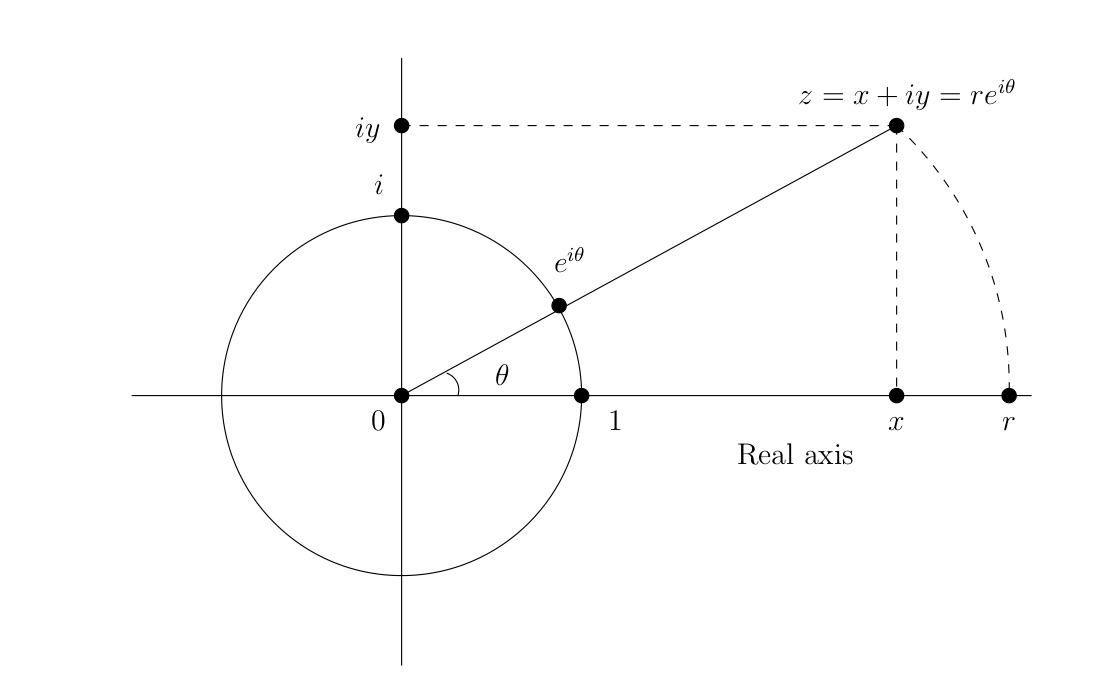
\includegraphics[width=1\linewidth]{images/zxyrtheta_clip.jpg}
\caption{Rectangular and polar forms for a complex number  \(z\)\label{x:figure:zxyrthetafig}}
\end{figure}
\end{subsectionptx}
%
%
\typeout{************************************************}
\typeout{Subsection 0.1.5 Conjugation}
\typeout{************************************************}
%
\begin{subsectionptx}{Conjugation}{}{Conjugation}{}{}{g:subsection:idp140657216892768}
The \terminology{conjugate} of the complex number \(z=x+iy=re^{i\theta}\), denoted \(\overline{z}\) or \(z^\ast\), is defined to be \(z^\ast = x-iy =
re^{-i\theta}\). Geometrically, \(z^\ast\) is the reflection of \(z\) across the real axis (the \(x\)-axis) in \(\R^2\). Here are some relations involving conjugates.%
\begin{align}
\re(z) \amp = \frac{z + z^\ast}{2}\label{x:mrow:realpartformula}\\
\im(z) \amp = \frac{z - z^\ast}{2i}\label{x:mrow:imagpartformula}\\
|z|^2 \amp = zz^\ast\label{x:mrow:zzbarisnormsq}\\
2\arg z \amp = \frac{z}{z^\ast} \;\;\text{(for )}\label{g:mrow:idp140657216900096}\\
\frac{1}{z}
\amp = \frac{z^\ast}{zz^\ast}= \frac{z^\ast}{|z|^2} \;\;\text{(for )}\label{g:mrow:idp140657216900976}\\
(zw)^\ast \amp = z^\ast w^\ast\label{g:mrow:idp140657216901888}
\end{align}
%
\end{subsectionptx}
%
%
\typeout{************************************************}
\typeout{Exercises 0.1.6 Exercises}
\typeout{************************************************}
%
\begin{exercises-subsection}{Exercises}{}{Exercises}{}{}{g:exercises:idp140657216902768}
\begin{divisionexercise}{1}{}{}{g:exercise:idp140657216903344}%
What is the difference between polar coordinates and polar form? What is the difference between rectangular coordinates and rectangular form?  Write formulas for converting from polar to rectangular coordinates and vice-versa.\par\smallskip%
\noindent\textbf{Solution}.\hypertarget{g:solution:idp140657216904256}{}\quad{}Let \(z\) be a complex number, let \(x=\re(z)\), \(y=\im(z)\), \(r=|z|\) and \(\theta = \arg(z)\).  The pair \((r,\theta)\) is called the polar coordinates for \(z\), while the expression \(re^{i\theta}\) is called the polar form for \(z\).  The pair \((x,y)\) is called the rectangular coordinates for \(z\), while the expression \(x+iy\) is called the rectangular form for \(z\).%
\par
To convert from polar to rectangular, use the equations \(x=r\cos \theta,
y=r\sin \theta\) (show sketches to explain these formulas).  To convert from rectangular to polar, use \(r=\sqrt{x^2+y^2}\) and \(\tan \theta =
y/x\).  For the last equation, you must use judgment when \(x=0\) to decide whether \(\theta\) should be \(\pi/2\) or \(-\pi/2\).  You must also use judgment when calculating \(\theta = \arctan (y/x)\). The standard codomain for \(\arctan\) is the interval \((\pi/2,\pi/2)\), so you need to use \(\theta = \arctan (y/x) + \pi\) for \(x\lt 0\).%
\end{divisionexercise}%
\begin{divisionexercise}{2}{}{}{g:exercise:idp140657216916576}%
Express each of the following in rectangular and polar form. %
\begin{enumerate}[label=(\alph*)]
\item{}\(3(2-i) + 6(1+i)\) \textbf{Answer}.\quad{}\(12+3i=\sqrt{153}\;e^{i\arctan(1/4)}\)%
\item{}\(\left(2e^{i\pi/6}\right)\left(3e^{-i\pi/3}\right)\) \textbf{Answer}.\quad{}\(6e^{-i\pi/6}=3\sqrt{3}-3i\)%
\item{}\((2+3i)(4-i)\) \textbf{Answer}.\quad{}\(11+10i=\sqrt{221}\;e^{i\arctan(10/11)}\)%
\item{}\((1+i)^3\) \textbf{Answer}.\quad{}\(-2+2i=2\sqrt{2}\;e^{i3\pi/4}\)%
\end{enumerate}
\end{divisionexercise}%
\begin{divisionexercise}{3}{}{}{g:exercise:idp140657216923536}%
Prove the following property of norm. \begin{assemblage}{The triangle inequality.}{g:assemblage:idp140657216924112}%
For any two complex numbers \(z,w\), we have%
\begin{equation*}
|z+w|\leq |z|+|w|.
\end{equation*}
%
\end{assemblage}
\par\smallskip%
\noindent\textbf{Solution}.\hypertarget{g:solution:idp140657216926240}{}\quad{}The simplest approach is geometric: Sketch the parallelogram for vector addition and use the fact that the length of any side of a triangle is less than the sum of the lengths of the other two sides.\end{divisionexercise}%
\begin{divisionexercise}{4}{}{}{g:exercise:idp140657216926992}%
Prove \hyperref[x:mrow:zzbarisnormsq]{Equation~(\ref{x:mrow:zzbarisnormsq})}.\par\smallskip%
\noindent\textbf{Solution}.\hypertarget{g:solution:idp140657216928336}{}\quad{}Let \(z=re^{i\theta}\).  Then \(\overline{z}=re^{-i\theta}\), and we have%
\begin{align*}
z\overline{z} \amp = re^{i\theta}re^{-i\theta}\\
\amp = r^2 e^0\\
\amp = r^2 = |z|^2.
\end{align*}
\end{divisionexercise}%
\begin{divisionexercise}{5}{}{}{g:exercise:idp140657216931456}%
Let \(p\) and \(q\) be complex numbers.  Prove that the distance (ordinary distance between points in the plane) between \(p\) and \(q\) is \(|p-q|\).\par\smallskip%
\noindent\textbf{Hint}.\hypertarget{g:hint:idp140657216934176}{}\quad{}Hint: Use rectangular form.\par\smallskip%
\noindent\textbf{Solution}.\hypertarget{g:solution:idp140657216934608}{}\quad{}Let \(p=a+ib\) and \(q=c+id\). We have%
\begin{align*}
|p-q| \amp = |(a+ib)-(c+id)| \\
\amp = |(a-c)+i(b-d)|\\
\amp = \sqrt{(a-c)^2 + (b-d)^2}.
\end{align*}
The latter expression is the distance from \(p\) to \(q\), so we are done.\end{divisionexercise}%
\begin{divisionexercise}{6}{}{}{g:exercise:idp140657216938608}%
Express each of the following in rectangular and polar form. %
\begin{enumerate}[label=(\alph*)]
\item{}\(\displaystyle \frac{2+i}{3-i}\) \textbf{Answer}.\quad{}\(\displaystyle \frac{1}{2} + \frac{1}{2}i=\frac{\sqrt{2}}{2}e^{i\pi/4}\)%
\item{}\(\displaystyle \frac{1+2i}{1-2i}\) \textbf{Answer}.\quad{}\(\displaystyle -\frac{3}{5} +\frac{4}{5}i=e^{i(\arctan(-4/3)+\pi)}\)%
\item{}\(\displaystyle \frac{2e^{i\pi/4}}{3e^{-i\pi/2}}\) \textbf{Answer}.\quad{}\(\displaystyle \frac{2}{3}e^{i3\pi/4}=-\frac{\sqrt{2}}{3} + \frac{\sqrt{2}}{3}i\)%
\end{enumerate}
\end{divisionexercise}%
\begin{divisionexercise}{7}{}{}{g:exercise:idp140657216944160}%
Verify the formulas \hyperref[x:mrow:realpartformula]{(\ref{x:mrow:realpartformula})} and \hyperref[x:mrow:imagpartformula]{(\ref{x:mrow:imagpartformula})}.\par\smallskip%
\noindent\textbf{Solution}.\hypertarget{g:solution:idp140657216945888}{}\quad{}Let \(z=x+iy\).  Then we have %
\begin{itemize}[label=\textbullet]
\item{}\(\displaystyle \frac{z+\overline{z}}{2}= \frac{2x}{2}=x=\re(z)\), and%
\item{}\(\displaystyle
\frac{z-\overline{z}}{2i}=\frac{2iy}{2i}=y=\im(z)\).%
\end{itemize}
\end{divisionexercise}%
\begin{divisionexercise}{8}{}{}{g:exercise:idp140657216948928}%
Given a nonzero complex number \(z\), explain why \(z\) has exactly two square roots, and explain how to find them.\par\smallskip%
\noindent\textbf{Solution}.\hypertarget{g:solution:idp140657216950528}{}\quad{}Since squaring a number squares the norm and doubles the argument, a square root can be found by taking the square root of the norm and dividing the argument by two.  That is, for \(z=re^{i\theta}\), a square root of \(z\) is \(\sqrt{r}e^{i\theta/2}\).  Another square root of \(z\) is the negative of that expression.  Any other square root of \(z\) would have to have norm \(\sqrt{|z|}\) and argument \(\theta/2\) plus or minus an integer multiple of \(\pi\), so these must be all the square roots of \(z\).\end{divisionexercise}%
\begin{divisionexercise}{9}{}{}{g:exercise:idp140657216955184}%
Find all complex solutions of the following equations. %
\begin{enumerate}[label=(\alph*)]
\item{}\(\displaystyle z^2 + 3z + 5 = 0\) \textbf{Answer}.\quad{}\(\displaystyle -\frac{3}{2} \pm i\frac{\sqrt{11}}{2}\)%
\item{}\((z - i)(z + i) = 1\) \textbf{Answer}.\quad{}\(0\)%
\item{}\(\displaystyle \frac{2z + i}{-z+3i} = z\) \textbf{Answer}.\quad{}\(\displaystyle (1/2)[(-2 \pm 281^{1/4}\cos \varphi) + i(3 \pm
281^{1/4}\sin \varphi)]\), where \(\varphi=(\arctan(16/5)+\pi)/2\)%
\end{enumerate}
\end{divisionexercise}%
\begin{divisionexercise}{10}{}{}{g:exercise:idp140657216961232}%
Use the fact that \(e^{ia}e^{ib}=e^{i(a+b)}\) together with Euler's formula \(e^{i\theta}=\cos\theta + i\sin\theta\) to derive the trigonometric angle sum formulas below.%
\begin{align*}
\cos(a+b) \amp = \cos a \cos b -\sin a \sin b\\
\sin(a+b) \amp = \cos a \sin b + \sin a \cos b
\end{align*}
\par\smallskip%
\noindent\textbf{Solution}.\hypertarget{g:solution:idp140657216964240}{}\quad{}Using Euler's formula for the first equality below, and then using complex multiplication for the second equality, we have%
\begin{align}
e^{ia}e^{ib} \amp = (\cos a + i\sin a)(\cos b + i\sin b)\notag\\
\amp = (\cos a\cos b - \sin a \sin b) + i(\cos a \sin b + \sin a\cos b).\tag{\(\star\)}\label{x:mrow:localtag1}
\end{align}
On the other hand, Euler's formula also gives%
\begin{gather}
e^{i(a+b)}= \cos(a+b) + i\sin
(a+b).\tag{\(\star\star\)}\label{x:mrow:localtag2}
\end{gather}
Equating real and and imaginary parts of \hyperref[x:mrow:localtag1]{(\ref{x:mrow:localtag1})} and \hyperref[x:mrow:localtag2]{(\ref{x:mrow:localtag2})} gives the desired trigonometric identities.\end{divisionexercise}%
\end{exercises-subsection}
\end{sectionptx}
%
%
\typeout{************************************************}
\typeout{Section 0.2 Equivalence Relations}
\typeout{************************************************}
%
\begin{sectionptx}{Equivalence Relations}{}{Equivalence Relations}{}{}{g:section:idp140657216969856}
\begin{introduction}{}%
section about equivalence relations here\end{introduction}%
%
%
\typeout{************************************************}
\typeout{Subsection 0.2.1 Definitions}
\typeout{************************************************}
%
\begin{subsectionptx}{Definitions}{}{Definitions}{}{}{g:subsection:idp140657216971024}
an equivalence relation is%
\end{subsectionptx}
\end{sectionptx}
%
%
\typeout{************************************************}
\typeout{Section 0.3 Modular Arithmetic}
\typeout{************************************************}
%
\begin{sectionptx}{Modular Arithmetic}{}{Modular Arithmetic}{}{}{g:section:idp140657216972688}
\begin{introduction}{}%
section about modular arithmetic here\end{introduction}%
%
%
\typeout{************************************************}
\typeout{Subsection 0.3.1 Definitions}
\typeout{************************************************}
%
\begin{subsectionptx}{Definitions}{}{Definitions}{}{}{g:subsection:idp140657216973840}
the integers are awesome%
\end{subsectionptx}
\end{sectionptx}
%
%
\typeout{************************************************}
\typeout{Section 0.4 Linear Algebra Basics}
\typeout{************************************************}
%
\begin{sectionptx}{Linear Algebra Basics}{}{Linear Algebra Basics}{}{}{g:section:idp140657216975504}
\begin{introduction}{}%
section about basics of linear algebra\end{introduction}%
%
%
\typeout{************************************************}
\typeout{Subsection 0.4.1 Definitions}
\typeout{************************************************}
%
\begin{subsectionptx}{Definitions}{}{Definitions}{}{}{g:subsection:idp140657216976656}
a vector is a thing%
\end{subsectionptx}
\end{sectionptx}
\end{chapterptx}
%
%
\typeout{************************************************}
\typeout{Chapter 1 Algebra}
\typeout{************************************************}
%
\begin{chapterptx}{Algebra}{}{Algebra}{}{}{x:chapter:algebra_chapter}
\begin{introduction}{}%
This is algebra.\end{introduction}%
%
%
\typeout{************************************************}
\typeout{Section 1.1 Examples of groups}
\typeout{************************************************}
%
\begin{sectionptx}{Examples of groups}{}{Examples of groups}{}{}{g:section:idp140657186746672}
\begin{introduction}{}%
hiya\end{introduction}%
%
%
\typeout{************************************************}
\typeout{Subsection 1.1.1 }
\typeout{************************************************}
%
\begin{subsectionptx}{}{}{}{}{}{g:subsection:idp140657219309744}
Examples:%
\begin{itemize}[label=\textbullet]
\item{}permutation groups%
\item{}symmetries of planar figures, \(R_\theta\), \(F_L\) notation%
\item{}\(2\times 2\) matrix groups%
\item{}integers, integers mod \(n\)%
\end{itemize}
%
\end{subsectionptx}
\end{sectionptx}
%
%
\typeout{************************************************}
\typeout{Section 1.2 Definitions and properties for groups}
\typeout{************************************************}
%
\begin{sectionptx}{Definitions and properties for groups}{}{Definitions and properties for groups}{}{}{g:section:idp140657219402912}
\begin{introduction}{}%
hiya\end{introduction}%
%
%
\typeout{************************************************}
\typeout{Subsection 1.2.1 }
\typeout{************************************************}
%
\begin{subsectionptx}{}{}{}{}{}{g:subsection:idp140657219412048}
define group and tie formal definition to examples from previous section, use more vocabulary such as \emph{subgroup}%
\end{subsectionptx}
\end{sectionptx}
%
%
\typeout{************************************************}
\typeout{Section 1.3 Group homomorphisms}
\typeout{************************************************}
%
\begin{sectionptx}{Group homomorphisms}{}{Group homomorphisms}{}{}{g:section:idp140657219433584}
\begin{introduction}{}%
hiya\end{introduction}%
%
%
\typeout{************************************************}
\typeout{Subsection 1.3.1 }
\typeout{************************************************}
%
\begin{subsectionptx}{}{}{}{}{}{g:subsection:idp140657219455568}
define vocabulary including homomorphism, isomorphism, kernel, image%
\par
develop properties of normal subgroup%
\end{subsectionptx}
\end{sectionptx}
%
%
\typeout{************************************************}
\typeout{Section 1.4 Fundamental theorems of groups}
\typeout{************************************************}
%
\begin{sectionptx}{Fundamental theorems of groups}{}{Fundamental theorems of groups}{}{}{g:section:idp140657219484224}
\begin{introduction}{}%
hiya\end{introduction}%
%
%
\typeout{************************************************}
\typeout{Subsection 1.4.1 }
\typeout{************************************************}
%
\begin{subsectionptx}{}{}{}{}{}{g:subsection:idp140657219510448}
group mod kernel is isomorphic to the image%
\par
Lagrange's theorem as a consequence for a sepcial case%
\end{subsectionptx}
\end{sectionptx}
%
%
\typeout{************************************************}
\typeout{Section 1.5 Group actions}
\typeout{************************************************}
%
\begin{sectionptx}{Group actions}{}{Group actions}{}{}{g:section:idp140657219561600}
\begin{introduction}{}%
hiya\end{introduction}%
%
%
\typeout{************************************************}
\typeout{Subsection 1.5.1 }
\typeout{************************************************}
%
\begin{subsectionptx}{}{}{}{}{}{g:subsection:idp140657219603456}
defintions: action, orbit, stabilizer%
\par
orbit-stabilizer theorem(s), applications%
\end{subsectionptx}
\end{sectionptx}
\end{chapterptx}
%
%
\typeout{************************************************}
\typeout{Chapter 2 Geometry}
\typeout{************************************************}
%
\begin{chapterptx}{Geometry}{}{Geometry}{}{}{x:chapter:geometry_chapter}
\begin{introduction}{}%
This is geometry. We will spend most of our time on planar geometries.\end{introduction}%
%
%
\typeout{************************************************}
\typeout{Section 2.1 Euclidean geometry}
\typeout{************************************************}
%
\begin{sectionptx}{Euclidean geometry}{}{Euclidean geometry}{}{}{g:section:idp140657235278464}
\begin{introduction}{}%
hiya\end{introduction}%
%
%
\typeout{************************************************}
\typeout{Subsection 2.1.1 }
\typeout{************************************************}
%
\begin{subsectionptx}{}{}{}{}{}{g:subsection:idp140657235279488}
Euclidean geometry in the plane via algebra of the complex numbers%
\end{subsectionptx}
\end{sectionptx}
%
%
\typeout{************************************************}
\typeout{Section 2.2 Möbius geometry}
\typeout{************************************************}
%
\begin{sectionptx}{Möbius geometry}{}{Möbius geometry}{}{}{g:section:idp140657235280672}
\begin{introduction}{}%
hiya\end{introduction}%
%
%
\typeout{************************************************}
\typeout{Subsection 2.2.1 }
\typeout{************************************************}
%
\begin{subsectionptx}{}{}{}{}{}{g:subsection:idp140657235281792}
Möbius geometry as a \(GL(2,\C)\) action on \(\C\)%
\end{subsectionptx}
\end{sectionptx}
%
%
\typeout{************************************************}
\typeout{Section 2.3 Möbius geometry as projective geometry}
\typeout{************************************************}
%
\begin{sectionptx}{Möbius geometry as projective geometry}{}{Möbius geometry as projective geometry}{}{}{g:section:idp140657235283872}
\begin{introduction}{}%
hiya\end{introduction}%
%
%
\typeout{************************************************}
\typeout{Subsection 2.3.1 }
\typeout{************************************************}
%
\begin{subsectionptx}{}{}{}{}{}{g:subsection:idp140657235285008}
Möbius geometry as projective geometry of the projective space of \(\C^2\), introduce stereographic projection as a tool%
\end{subsectionptx}
\end{sectionptx}
%
%
\typeout{************************************************}
\typeout{Section 2.4 Hyperbolic geometry}
\typeout{************************************************}
%
\begin{sectionptx}{Hyperbolic geometry}{}{Hyperbolic geometry}{}{}{g:section:idp140657235286784}
\begin{introduction}{}%
hiya\end{introduction}%
%
%
\typeout{************************************************}
\typeout{Subsection 2.4.1 }
\typeout{************************************************}
%
\begin{subsectionptx}{}{}{}{}{}{g:subsection:idp140657235287904}
Hyperbolic geometry as a subgeometry of Möbius geometry%
\end{subsectionptx}
\end{sectionptx}
%
%
\typeout{************************************************}
\typeout{Section 2.5 Elliptic geometry}
\typeout{************************************************}
%
\begin{sectionptx}{Elliptic geometry}{}{Elliptic geometry}{}{}{g:section:idp140657235289184}
\begin{introduction}{}%
hiya\end{introduction}%
%
%
\typeout{************************************************}
\typeout{Subsection 2.5.1 }
\typeout{************************************************}
%
\begin{subsectionptx}{}{}{}{}{}{g:subsection:idp140657235290304}
Elliptic geometry as a subgeometry of Möbius geometry%
\end{subsectionptx}
\end{sectionptx}
%
%
\typeout{************************************************}
\typeout{Section 2.6 Projective geometry}
\typeout{************************************************}
%
\begin{sectionptx}{Projective geometry}{}{Projective geometry}{}{}{g:section:idp140657235291584}
\begin{introduction}{}%
hiya\end{introduction}%
%
%
\typeout{************************************************}
\typeout{Subsection 2.6.1 }
\typeout{************************************************}
%
\begin{subsectionptx}{}{}{}{}{}{g:subsection:idp140657235292704}
Projective (real and complex) geometry%
\end{subsectionptx}
\end{sectionptx}
%
%
\typeout{************************************************}
\typeout{Section 2.7 The quaternions}
\typeout{************************************************}
%
\begin{sectionptx}{The quaternions}{}{The quaternions}{}{}{g:section:idp140657235293968}
\begin{introduction}{}%
hiya\end{introduction}%
%
%
\typeout{************************************************}
\typeout{Subsection 2.7.1 }
\typeout{************************************************}
%
\begin{subsectionptx}{}{}{}{}{}{g:subsection:idp140657235295088}
algebra of rotations in 3-dimensional Euclidean space%
\end{subsectionptx}
\end{sectionptx}
\end{chapterptx}
%
%
\typeout{************************************************}
\typeout{Chapter 3 More Topics}
\typeout{************************************************}
%
\begin{chapterptx}{More Topics}{}{More Topics}{}{}{g:chapter:idp140657219220528}
\begin{introduction}{}%
This is more topics.\end{introduction}%
%
%
\typeout{************************************************}
\typeout{Section 3.1 Further topics}
\typeout{************************************************}
%
\begin{sectionptx}{Further topics}{}{Further topics}{}{}{g:section:idp140657219225728}
%
%
\typeout{************************************************}
\typeout{Subsection 3.1.1 }
\typeout{************************************************}
%
\begin{subsectionptx}{}{}{}{}{}{g:subsection:idp140657219193728}
more algebra topics: group classification problems, Sylow theorems, fundamental theorem of finitely generated Abelian groups, more structures like rings, fields, vector spaces and modules, some properties%
\par
more geometry topics: finite geometries, using stereographic projection to count Pythagorean triples%
\end{subsectionptx}
\end{sectionptx}
\end{chapterptx}
%
\backmatter
%
%
%% A lineskip in table of contents as transition to appendices, backmatter
\addtocontents{toc}{\vspace{\normalbaselineskip}}
%
%
%% The index is here, setup is all in preamble
\printindex
%
\end{document}
